\chapter{Dasar Teori}
\label{chap: dasarTeori}

\section{CodeIgniter}
\label{sec: codeigniter}

	\textit{CodeIgniter} merupakan sebuah \textit{framework} pemrograman \textit{web} dengan menggunakan bahasa php. \textit{CodeIgniter} (CI) akan membantu mengurangi jumlah pengerjaan kode yang harus diketik, mempermudah pembacaan dan pembaharuan \textit{script}, membantu penyusunan struktur yang jelas dan rinci, mendisiplinkan diri dalam pengerjaan \textit{coding} dan memperkuat hasil tanpa disadari.
	
	
	\subsection{Keistimewaan CI}
	\label{sub: KeistimewaanCI}
	CodeIgniter memiliki beberapa keistimewaan antara lain:
	\begin{enumerate}
		\item Menghemat waktu pengembangan
		\item \textit{Reuse of code} (pemakaian kembali kode yang sudah ada)
		\item Adanya bantuan dari komunitas CI
	\end{enumerate}	
	
	
	\subsection{Model, View, dan Controller(MVC) pada CI}
	\label{sub: mvc}
	
	Konsep MVC adalah konsep pemisahan antara logic dengan tampilan dan database. Manfaat konsep ini adalah, membuat coding logic lebih simple, karena sudah di pisah dengan code untuk tampilan dan membuat programmer dapat bekerja secara terpisah dengan designer.
	CodeIgniter sendiri dibangun menggunakan konsep \textit{Model-View-Controller development pattern}. Manfaat konsep MVC ini adalah memudahkan logika dalam \textit{coding} aplikasi tersebut dan memudahkan pengembangan sistem yang sudah ada.
	\begin{itemize}
		\item \textit{Model} = \textit{Model} berhubungan dengan data dan interaksi ke \textit{database} atau \textit{webservice}. \textit{Model} juga merepresentasikan struktur data dari aplikasi yang bisa berupa basis data maupun data lain, misalnya dalam bentuk file teks, \textit{file} XML maupun webservice. Biasanya di dalam model akan berisi class dan fungsi untuk mengambil, melakukan update dan menghapus data website. Sebuah
		aplikasi web biasanya menggunakan basis data dalam menyimpan data, maka pada bagian \textit{Model} biasanya akan berhubungan dengan perintah-perintah \textit{query} SQL.
		\item \textit{View} = \textit{View} berhubungan dengan segala sesuatu yang akan ditampilkan ke \textit{end-user}. Bisa berupa halaman web, rss, javascript dan lain-lain. Di dalam \textit{view} hanya berisi variabel-variabel yang berisi data yang siap ditampilkan. View dapat dikatakan sebagai halaman website yang dibuat dengan	menggunakan HTML dan bantuan CSS atau JavaScript. \textit{View} hanya dikhususkan untuk menampilkan data-data hasil dari \textit{model} dan \textit{controller}
		\item \textit{Controller} = \textit{Controller} bertindak sebagai penghubung data dan \textit{view}. Di dalam \textit{Controller} inilah terdapat kelas-kelas dan fungsi-fungsi yang memproses permintaan dari View ke dalam struktur data di dalam \textit{Model}. \textit{Controller} juga tidak boleh berisi kode untuk mengakses basis data karena tugas mengakses data telah diserahkan kepada \textit{model}. Tugas \textit{controller} adalah menyediakan berbagai variabel yang akan ditampilkan di \textit{view}, memanggil \textit{model} untuk melakukan akses ke basis data, menyediakan penanganan kesalahan/\textit{error}, mengerjakan proses logika dari aplikasi serta melakukan validasi atau cek terhadap \textit{input}.
	
	\end{itemize}
	
	Berikut ini adalah alur proses konsep MVC:
	
	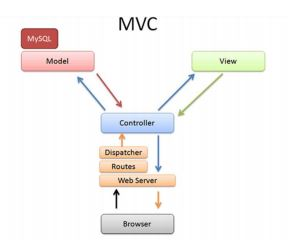
\includegraphics[scale=1.00]{Gambar/konsepMVC}
	
	CI menerapkan pola MVC yang flexible, karena model dapat tidak di gunakan. Anda dapat hanya menggunakan Controller dan View saja dalam menggunakan CI
	tanpa Model. Jika anda tidak memerlukan pemisahan di dalam struktur data dan database atau menganggap penggunaan model hanya menambah kompleks aplikasi dengan keuntungan yang kurang sebanding, maka anda dapat tidak menggunakan model.
	
	\subsection{Struktur CI}
	\label{sub: strukturCI}
	CI adalah sebuah php framework yang berupa kumpulan folder dan file php, java script,css,txt dan file berbasis web lainnya dengan setting tertentu untuk menggunakannya dan menyediakan library dan helper yang dapat di manfaatkan di dalam pemrograman php. CI di jalankan under web dan harus dengan web server. Program CI cukup di letakkan di bawah folder directory web server anda.
	Berikut adalah struktur file CI :
	
	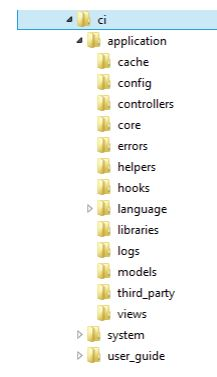
\includegraphics[scale=1]{Gambar/strukturCI}
		

\section{AngularJS}
\label{sec: angularJS}
	
	AngularJS merupakan \textit{framework javascript} berbasis \textit{open-source} yang dirilis oleh Google pada tahun 2009. AngularJS sendiri merupakan jawaban dari banyak tantangan pemakaian web yang memerlukan pengaplikasian suatu fungsi tanpa berganti halaman. Jika anda merujuk pada situs resmi AngularJS yaitu http://angularjs.org maka anda akan dapat membaca sebuah tagline "HTML Enchanced for Web Apps". Tag line tersebut mengartikan bahwa pemakaian angularJS merupakan pemakaian HTML yang telah ditingkatkan fungsinya untuk membangun sebuah aplikasi dalam web.
	
	HTML merupakan alat yang digunakan untuk membangun web statik sehingga membutuhkan bantuan dari alat lain untuk membuat sebuah aplikasi web pada HTML ini. Oleh sebab minat dan banyaknya permintaan dari developer web untuk membuat aplikasi web dengan mudah, maka Google meresmikan AngularJS pada tahun 2009 yang lalu.
	
	AngularJS bukan merupakan pustaka (library) javascript melainkan sebuah framework yang solid untuk membangun web app, seperti framework javascript pada umumnya AngularJS mengadopsi konsep MVC (Model, View, Controller), meskipun menggunakan implementasi yang berbeda dengan konsep asli MVC.
	
\subsection{Keistimewaan AngularJS}
\label{sub: keistimewaanAngularJS}
	Keistimewaan penggunaan AngularJS sangatlah banyak. Berikut beberapa diantaranya:
	
\subsubsection{Two way data-binding}
\label{sub: twoWayDataBinding}

	Two way data-binding merupakan mekanisme sinkronisasi otomatis antara Controller dan View. Gampangnya, ketika ada perubahan pada Model yang berasal dari View, Angular secara otomatis membuat perubahan pada Controller. Begitu pula sebaliknya. Hal ini terjadi secara otomatis, jadi kita tidak perlu menuliskan kode secara manual untuk mencapai mekanisme ini.

\subsubsection{Mengajari browsers dengan sintak HTML baru}
\label{subsub: mengajariBrowsersDenganSintakHTMLBaru}

	HTML5 menawarkan sejumlah elemen baru semisal <video>, <section>, <article>, dsb. Nah dengan AngularJS, Kita bahkan dapat menambahkan lebih banyak lagi elemen-elemen baru yang akan dimengerti oleh browser, misal <draggable> membuat elemen bisa didrag, <zippy> membuat elemen semisal akordion, atau bahkan menggunakan bahasa indonesia seperti <sembunyikan> jika diklik akan menyembunyikan elemen (contoh saja, pada praktik gunakanlah bahasa inggris sebagai bahasa internasional). Fungsi ini disebut dengan istilah Directive. Kitalah yang bertanggungjawab membuat Directive tersebut bisa ditafsirkan oleh browser dengan menuliskan kode pada deklarasi Directive itu sendiri. Atau dengan kata lain, kita mengajari browser sintak HTML baru. Bahkan tidak terbatas pada elemen, kita bisa membuat Directive menggunakan attribute, HTML comment atau class.

\subsubsection{HTML Template}
\label{subsub: HTMLTemplate}

	Template yang digunakan AngularJS hanyalah HTML biasa dengan penambahan ekspresi (expression), sehingga kita tidak perlu menggunakan template engine khusus.

\subsubsection{Dependecy Injection (DI)}
\label{subsub: DI}

	Dependency Injection memungkinkan developer menulis beberapa komponen kode yang terpisah satu sama lain. Ketika memerlukan salah satu komponen, developer dapat memanggil komponen yang dibutuhkan tersebut dan dapat menggunakan fungsi yang tersedia. Fitur ini memudahkan developer dalam membuat komponen yang dapat dipakai berulang kali (reusable component)

\subsection{Komponen AngularJS}
\label{sub: komponenAngularJS}
	


\subsubsection{Model}
\label{subsub: model}

	Dalam pola MVC, Model merepresentasikan suatu set data yang digunakan oleh Controller dan View.Model dapat mendeteksi perubahan data dan memberikan notifikasi perubahan tersebut ke Controller dan View. Pada implementasi pasif, notifikasi perubahan dapat diabaikan. Untuk membuat Model di beberapa framework selain AngularJS diperlukan konstruktor khusus. Sedangkan Model pada AngularJS tidak memiliki konstruktor tersendiri dan tidak memerlukan inheritance dari Object Class tertentu. Model tidak memerlukan setter atau getter method khusus. Model bisa berupa primitive, object hash, atau full object. Dengan kata lain Model hanyalah javascript object biasa.

\subsubsection{Scope}
\label{sub: Scope}

	Scope merupakan perekat (glue) atau perantara antara Controller dengan View. Masing-masing controller memiliki scope atau lingkup sendiri.
	
\subsubsection{Controller}
\label{subsub: controller}

	Controller merupakan kode dibalik View. Kode pemrosesan dan logika ditaruh pada controller yang akan menghasilkan Model untuk ditampilkan pada View.

\subsubsection{View}
\label{subsub: view}

	View adalah apa yang terlihat oleh pengguna. Dimulai dari sebuah template kemudian digabungkan dengan Model lalu browser melakukan proses rendering dan hasilnya ditampilkan ke pengguna. Template yang digunakan hanyalah sintak HTML (bukan HTML diselingi dengan markup khusus seperti pada template engine pada umumnya).

\subsubsection{Expression}
\label{subsub: expression}

	Expression merupakan kode snippet yang dapat kita tulis pada View. Expression berkaitan dengan mekanisme binding pada AngularJS, formatnya adalah sebagai berikut \{\{ expression \}\} Contoh :
	
	\begin{enumerate}
		\item "\{\{ 1+2 \}\}" , akan menampilkan angka 3 ke pengguna.
		\item \{\{ user.name \}\} , akan menampilkan nilai properti 'name' dari model 'user'
		\item \{\{ 1000 | currency \}\} , akan menampilkan angka 1000 dalam format mata uang (currency), keyword setelah tanda pipa ( | ) merupakan filter.
	\end{enumerate}

\subsubsection{Directive}
\label{subsub: directive}

	Directive merupakan cara untuk membuat sintak HTML baru yang akan dimengerti oleh browser. Directive dapat berupa elemen, attribute, HTML comment atau Class. Angular telah menyediakan beberapa directive bawaan yang penting dalam pengembangan web app. Beberepa directive bawaan Angular diantaranya ng-controller, ng-model, ng-repeat, ng-click dll. Kita dapat pula membuat custom directive dengan perilaku (behavior) tertentu seperti yang telah dijelaskan pada pembahasan Apa yang membuat AngularJS istimewa.
	
\section{Twitter Bootstrap}
\label{sec: bootstrap}

	Twitter Bootstrap adalah sebuah alat bantu untuk membuat sebuah tampilan halaman \textit{website} yang dapat mempercepat pekerjaan seorang pengembang \textit{website} ataupun pendesain halaman \textit{website}. Sesuai namanya, website yang dibuat dengan alat bantu ini memiliki tampilan halaman yang sama / mirip dengan tampilan halaman \textit{Twitter} atau desainer juga dapat mengubah tampilan halaman \textit{website} sesuai dengan kebutuhan.

	Twitter Bootstrap dibangun dengan teknologi HTML dan CSS yang dapat	membuat layout halaman website, tabel, tombol, form, navigasi, dan komponen	lainnya dalam sebuah website hanya dengan memanggil fungsi CSS (class) dalam berkas HTML yang telah didefinisikan. Selain itu juga terdapat komponen-komponen lainnya yang dibangun menggunakan JavaScript.
	
	\subsection{Struktur direktori Bootstrap}
	\label{sub: struturDirektoriBootstrap}
	
	Berikut adalah gambar struktur direktori dari \textit{Bootstrap}:
	
	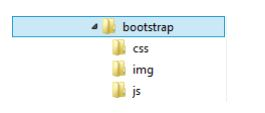
\includegraphics[scale= 1.0]{Gambar/strukturBootstrap}
	
	\subsection{Keuntungan menggunakan Bootstrap}
	\label{sub: keuntunganBootstrap}
	
	Penggunaan \textit{Twitter Bootstrap} tentu saja memiliki banyak keuntungan, diantaranya adalah:
	
	\begin{itemize}
		\item Memudahkan dalam mendesain website
		\item Responsif (mendukung segala macam layar dan \textit{device})
		\item Adanya dokumentasi yang cukup lengkap
		\item Mempunyai tampak yang elegan
	\end{itemize} 
	
	